\section{Test Driven Development}
\label{sub:test_driven_development}

For at sikre et simpelt program med få fejl, blev det planlagt at skrive kernefunktionerne i programmet udviklet jævnfør softwareudviklingsprocessen \enquote{Test Driven Development} (TDD).
I TDD skrives unit tests af en metode, før selve implementeringen af funktionen. Denne udviklingsprocess sikrer, at nye funktionaliteter ikke ødelægger de forud eksisterende \cite{martin2006agile}. Programmøren tvinges også til at tænke på, hvordan metoden bruges ved kald. Det sikrer hermed, at metoden er overskueligt konstrueret, således at den kan kaldes problemfrit. Et andet aspekt af TDD, er at testkoden tjener som dokumentation af den testede metodes funktionalitet. Tilgengæld riskeres et øget tidsforbrug, der dog muligvis kan fraskrives fejlfinding.

\section{Unit Testing i Microsoft Visual Studio}
\label{sub:unit_testing_i_microsoft_visual_studio}

Microsofts unit test framework for managed code er anvendt til unit testing. Frameworket kan teste \enquote{managed code}, som C\# falder ind under. Når tests er skrevet, kan Test Explorer i Visual Studio køre testene. Når testene er færdige, vil resultaterne blive præsenteret som \enquote{failed tests}, \enquote{passed tests}, \enquote{not run tests} og \enquote{skipped tests} \cite{msdn_unittest}.

Før der skrives unit tests, skal der oprettes et unit test projekt. Herefter kan der tilføjes klasser annoteret med \enquote{[TestClass]}. Inde i disse klasser, tilføjer man de metoder, annoteret med \enquote{[TestMethod]}, som skal køres. Et eksempel på en test metode, kan se i \cref{lst:simple_test}.
Alle tests til systemet kan findes på CD'en der afleveres som bilag.

\begin{lstlisting}[label=lst:simple_test, caption={Eksempel på testfunktion}]
  [TestMethod]
  public void SimpleTest()
  {
    int expected = 4;
    int actual = 2 + 2;

    Assert.AreEqual(expected, actual);
  }
\end{lstlisting}

\begin{figure}
  \centering
  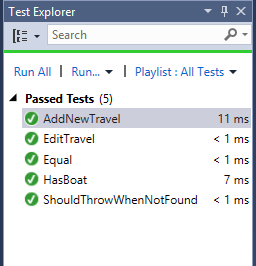
\includegraphics{test_explorer.png}
  \caption{Resultat af tests i Test Explorer i Visual Studio 2013}
  \label{fig:test_explorer}
\end{figure}

\section{Unit Testing i Løsningen}


I alt er der implementeret 25 unit tests til programmet, som alle kører succesfuldt, og kan findes i Visual Studio projektet \enquote{UnitTests}. De har til formål at teste forskellige klassers funktionaliteter. De første tests blev implementeret som en del af TDD forløbet, men det blev hurtigt avanceret, at teste klasser med eksterne moduler, som for eksempel persistenslaget. 

Efter udviklingen af SearchController klassen, blev der skrevet 9 grundige tests af denne klasse. Disse tests dækker alle funktionaliteter af SearchController klassen. Blandt andet testes det, om der kan søges i databasen på navnet af en bruger. Testen for dette ses i \cref{lst:test_searchcontroller}. Testen benytter metoden \enquote{simulateSearch} til at simulere brugerindtastning af \enquote{ali} i søgefeltet \enquote{navn}. Testen er en succes, hvis der returneres en liste, der kun indeholder personen \enquote{alice}. \enquote{alice} er i dette tilfælde den eneste person i databasen hvis navn indeholder \enquote{ali}.

\begin{lstlisting}[label=lst:test_searchcontroller, caption={Eksempel på testfunktion}]
[TestMethod]
public void SearchControllerTest_UserFoundByName()
{
        Action<IEnumerable<User>> action = delegate(IEnumerable<User> y)
        {
                Assert.IsTrue(y.Count() == 1 && y.Contains<User>(alice));

        };

        simulateSearch(action, "name", "ali");
}
\end{lstlisting}
